\documentclass[a4paper,11pt]{article}
\usepackage[left=1.5cm,right=1.5cm,top=2.0cm,bottom=2.8cm]{geometry}

\usepackage[ngerman,american]{babel}
\usepackage{graphicx}
\usepackage{amsmath}
\usepackage{amsthm}
\usepackage{amssymb}
\usepackage{listings}
\usepackage{epstopdf}
\usepackage{sidecap}
% \usepackage[FIGTOPCAP]{subfigure}
\usepackage{float}
\usepackage{color}
\usepackage[usenames,dvipsnames]{xcolor}
%\usepackage{empheq}
\usepackage[footnotesize,bf]{caption}
\usepackage{subcaption}
%\usepackage[framed,numbered,autolinebreaks,useliterate]{mcode}

\theoremstyle{definition}
\newtheorem{defi}{Definition}
\theoremstyle{plain}
\newtheorem{theo}[defi]{Theorem}
\theoremstyle{remark}
\newtheorem{remark}{Remark}

\providecommand{\abs}[1]{\lvert#1\rvert}
\providecommand{\norm}[1]{\lVert#1\rVert}

\renewcommand{\vec}[1]{\boldsymbol{#1}}

\title{Exercise 10}
\author{Philipp Hanslovsky, Robert Walecki}

\begin{document}


\lstloadlanguages{R} 
\lstset{language=R,
   %keywords={break,case,catch,continue,else,elseif,end,for,function,
   %   global,if,otherwise,persistent,return,switch,try,while},
   basicstyle=\ttfamily,
   keywordstyle=\color{blue},
   commentstyle=\color{green!40!black},
   stringstyle=\color{red},
   numbers=left,
   numberstyle=\tiny\color{white!50!black},
   stepnumber=1,
   numbersep=10pt,
   backgroundcolor=\color{white},
   tabsize=4,
   showspaces=false,
   showstringspaces=false,
   frame=single}


\maketitle

\section*{10.1}
\begin{align}
p(a, b) &= 0.048 + 0.096 = 0.144 \\
p(a)p(b) &= (0.192 + 0.064 + 0.048 + 0.096)(0.048 + 0.216 + 0.048 + 0.096) \\
&= 0.1632 \ne p(a, b) \\
p(a|c)p(b|c) &= \frac{p(a,c)p(b,c)}{p(c)^2} = \frac{0.16\cdot0.312}{0.52^2} = \frac{0.04992}{0.52^2} \\
p(a,b|c) &= \frac{p(a,b,c)}{p(c)} =\frac{0.096}{0.52} = \frac{0.04992}{0.52^2} = p(a|c)p(b|c) \\
p(a|\bar{c})p(b|\bar{c}) &= \frac{p(a,\bar{c})p(b,\bar{c})}{p(\bar{c})^2} = \frac{0.048^2}{0.48^2}(1+4)(1+1) = \frac{1}{100}\cdot10 = \frac{1}{10} \\
p(a,b|\bar{c}) &= \frac{p(a,b,\bar{c})}{p(\bar{c})} =\frac{0.048}{0.48} = \frac{1}{10} = p(a|\bar{c})p(b|\bar{c})
\end{align}

\begin{figure}[H]
\centering
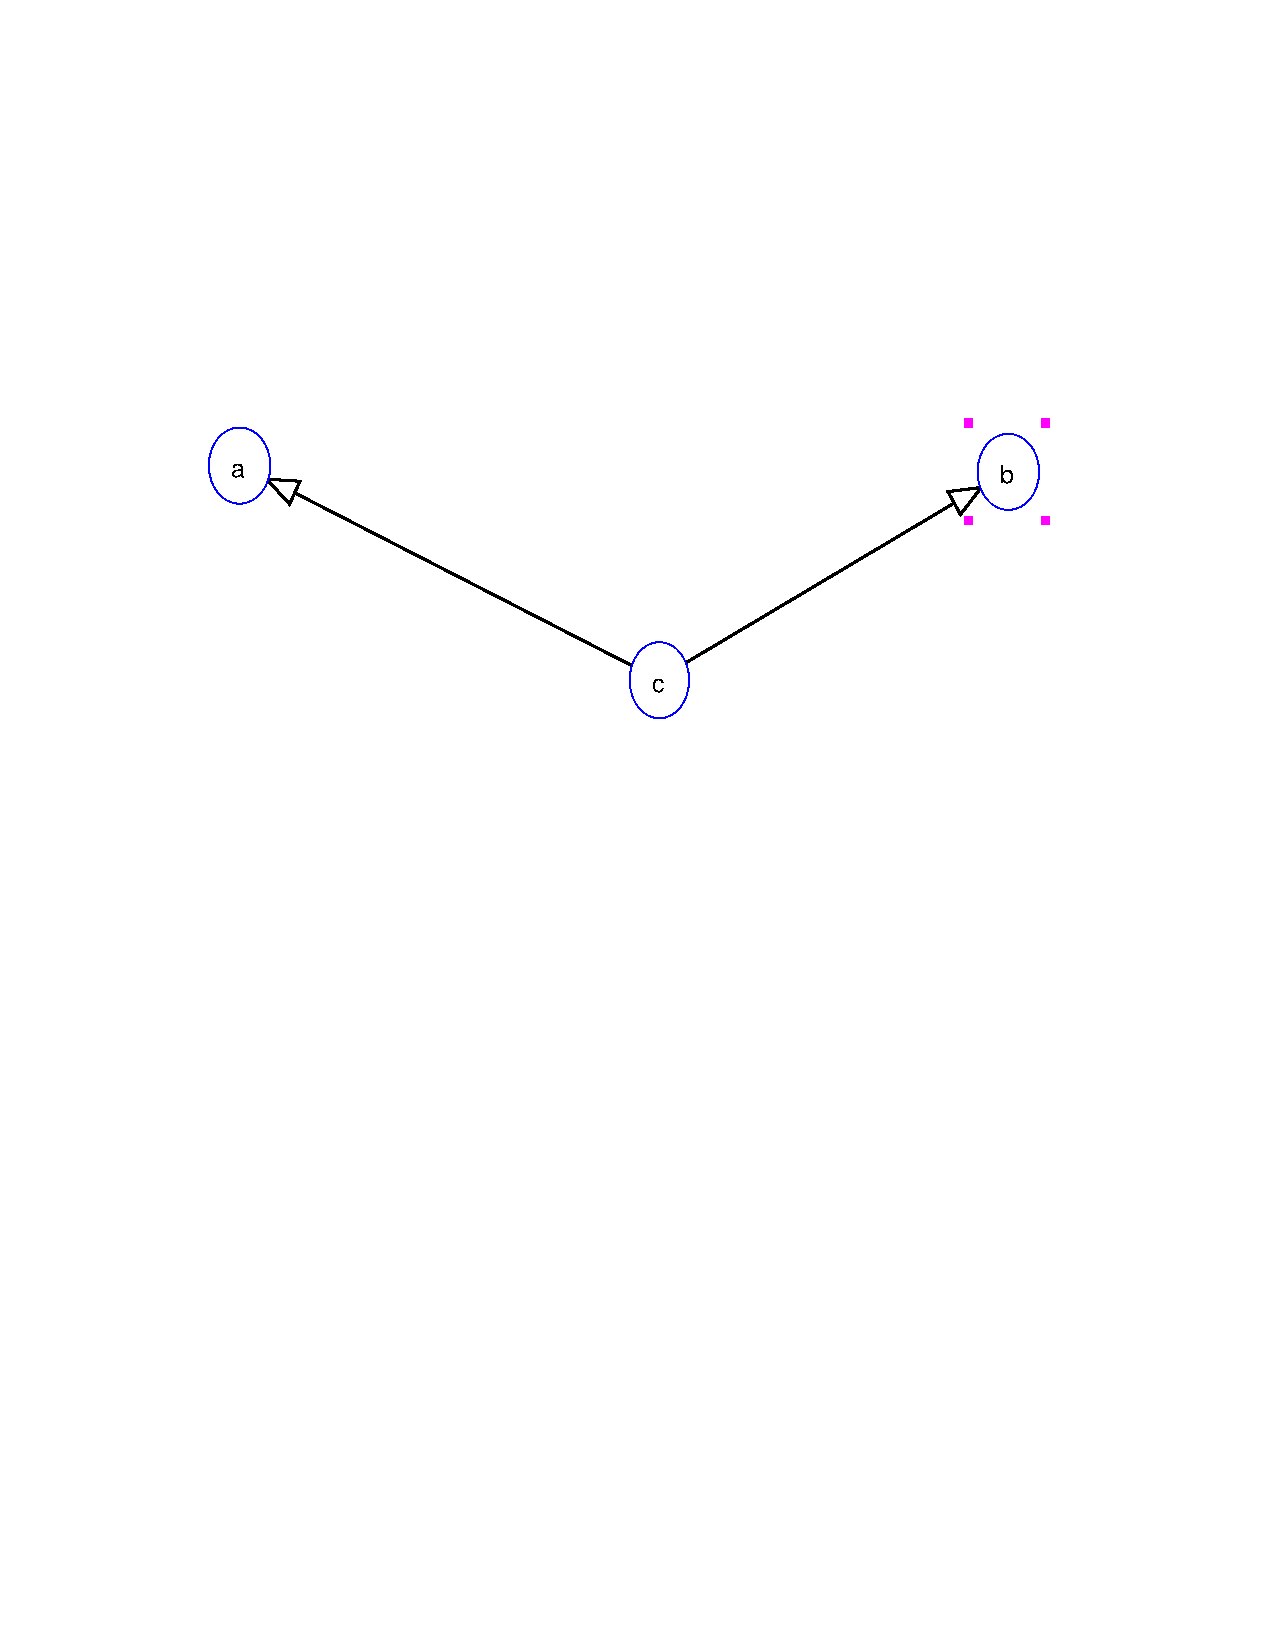
\includegraphics[width=0.6\textwidth]{out.pdf}
\caption{Graph for the given probability table}
\label{fig:graph}
\end{figure}

\begin{table}
\centering
\caption{Probability tables for the graph shown in fig \ref{fig:graph}}
\begin{tabular}{|c|c|l|}
\hline
a & c & $p(a|c)$ \\ \hline
0 & 0 & 0.5 \\ \hline
0 & 1 & 0.69 \\ \hline
1 & 0 & 0.5 \\ \hline
1 & 1 & 0.31 \\ \hline
\end{tabular}
~
\begin{tabular}{|c|c|l|}
\hline
a & c & $p(b|c)$ \\ \hline
0 & 0 & 0.8 \\ \hline
0 & 1 & 0.4 \\ \hline
1 & 0 & 0.2 \\ \hline
1 & 1 & 0.6 \\ \hline
\end{tabular}
~
\begin{tabular}{|c|l|}
\hline
c & $p(c)$ \\ \hline
0 & 0.52 \\ \hline
1 & 0.48 \\ \hline
\end{tabular}
\end{table}
Instead of seven parameters as before, only five parameters are needed now:
\begin{align}
p(c), p(a|c), p(a|\bar{c}), p(b,c), p(b|\bar{c})
\end{align}

\section*{10.2}

% Mach dei Zeug da rein, Robbat!
% ich klatsch dich weg
Def. d-separation:\\
A and B are d-separated by C if all paths from a vertex of A to a vertex of B are blocked.\\
\\
Def. Blocking:\\
A path between two vertices is blocked wrt C if it passes through a vertex v s.t.\\
      arrows are head-tail oder tail-tail and v is $\in$ C\\
      arrows are head-head and v as well as all of its descendants are ${\not\in}$ C\\
\\
to prove that A and B are not d-separated we have to find one path that is not blocked.\\
\\
1 is false\\
prof: \\
C - G - J - L is not blocked\\
\\
2 is false\\
prof: \\
J - G - C - H is not blocked\\
\\
3 is false\\
H - C - G - J - L - K - I - E is not blocked\\
\\
4 is galse\\
H - K - I - B - F - A is not blocked\\
\\
\section*{10.3.1}
The best fitting graph is graph \#4. The flaws of the others are:
In graph \#1 the ``Terminator 2'' node should be connected with the ``date plan'' node as we make our decision for the date plan based on the Terminator 2 rumor. The ``likes robot movies'' node should influence the date plan but only the girl's decision. Graph \#2 is the same as \#1 except the ``Terminator 3'' node's connection with the ``decision'' node is complete nonsense. The availability in local cinemas affects the date plan, not the decision. Graph \#3 is the same as \#1 except connecting the ``Terminator 3'' node with the ``Terminator 2'' node does not make any sense at all.

\section*{10.3.2}
\begin{table}[H]
\centering
\begin{tabular}{|c|c|c|c|}
\hline
observation & None & T2 = False & T2 = False, T3 = False \\ \hline
$p(decision = yes)$ & 0.51 & 0.45 & 0.45 \\ \hline
\end{tabular}
\end{table}

With the knowledge that the first guy proposed a walk in the park, the probability of her enjoying robot movies went down to 0.145. The probability that Terminator 3 is not running went up to 0.487. Knowing that she rejected the offer, the probability for her liking robot movies went down to 0.150.

\end{document}
